\documentclass{standalone}
\usepackage{xcolor}
\usepackage{tikz}
\usetikzlibrary{positioning}

\begin{document}
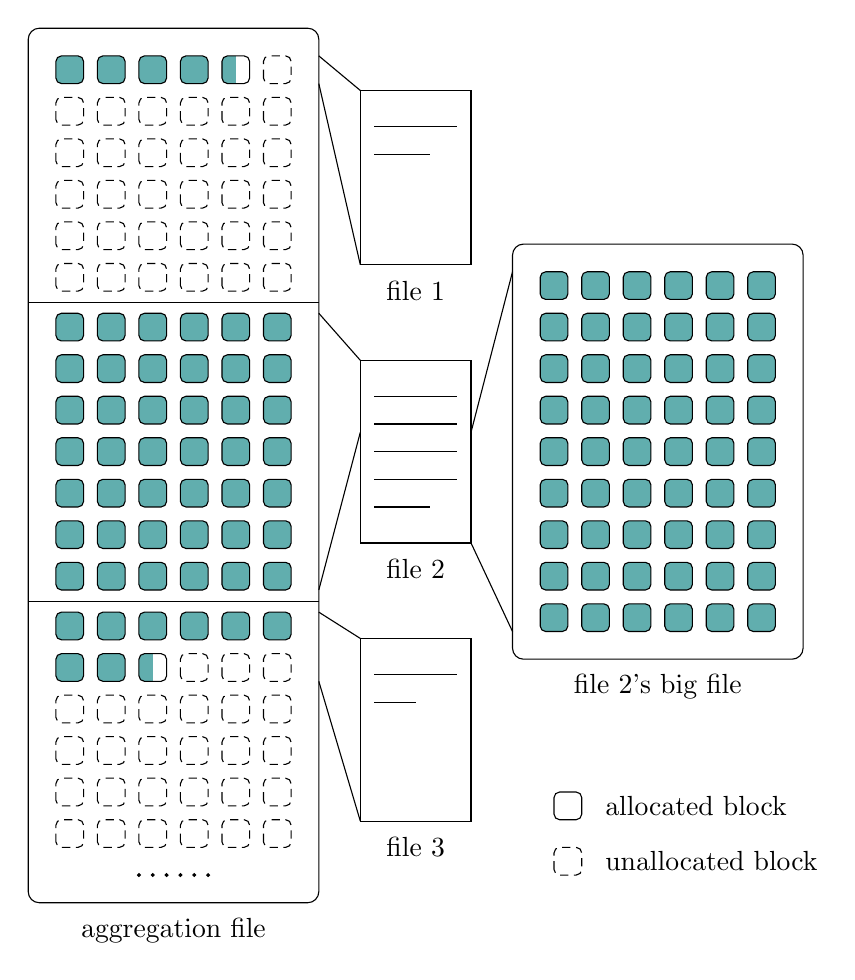
\begin{tikzpicture}[
  fill left/.style={path picture={\fill[#1] (path picture bounding box.south west)
  -- (path picture bounding box.north west)[rounded corners=0]
  -- (path picture bounding box.north)
  -- (path picture bounding box.south);}},
  x=1em,y=1em]

  \definecolor{main}{HTML}{61AEAE}

  % ------------------- blocks ----------------------
  \foreach \x in {0,...,5} {
    \foreach \y in {0,...,3} {
      \draw[rounded corners=2,densely dashed] (\x*1.5,\y*1.5) rectangle (\x*1.5+1,\y*1.5+1);
    }
  }
  \foreach \x in {0,...,5} {
    \draw[rounded corners=2,fill=main] (\x*1.5,7.5) rectangle (\x*1.5+1,8.5);
  }
  \draw[rounded corners=2,fill=main] (0,6) rectangle (1,7);
  \draw[rounded corners=2,fill=main] (1.5,6) rectangle (2.5,7);
  \draw[rounded corners=2,fill left=main] (3,6) rectangle (4,7);
  \draw[rounded corners=2,densely dashed] (4.5,6) rectangle (5.5,7);
  \draw[rounded corners=2,densely dashed] (6,6) rectangle (7,7);
  \draw[rounded corners=2,densely dashed] (7.5,6) rectangle (8.5,7);

  \draw (-1,8.9) -- (9.5,8.9);

  \foreach \x in {0,...,5} {
    \foreach \y in {6.2,...,12.2} {
      \draw[rounded corners=2,fill=main] (\x*1.5,\y*1.5) rectangle (\x*1.5+1,\y*1.5+1);
    }
  }

  \draw (-1,19.7) -- (9.5,19.7);

  \foreach \x in {0,...,5} {
    \foreach \y in {13.4,...,17.4} {
      \draw[rounded corners=2,densely dashed] (\x*1.5,\y*1.5) rectangle (\x*1.5+1,\y*1.5+1);
    }
  }
  \draw[rounded corners=2,fill=main] (0,27.6) rectangle (1,28.6);
  \draw[rounded corners=2,fill=main] (1.5,27.6) rectangle (2.5,28.6);
  \draw[rounded corners=2,fill=main] (3,27.6) rectangle (4,28.6);
  \draw[rounded corners=2,fill=main] (4.5,27.6) rectangle (5.5,28.6);
  \draw[rounded corners=2,fill left=main] (6,27.6) rectangle (7,28.6);
  \draw[rounded corners=2,densely dashed] (7.5,27.6) rectangle (8.5,28.6);

  \draw[fill] (3,-1)    circle[radius=0.05];
  \draw[fill] (3.5,-1)    circle[radius=0.05];
  \draw[fill] (4,-1)    circle[radius=0.05];
  \draw[fill] (4.5,-1)    circle[radius=0.05];
  \draw[fill] (5,-1)    circle[radius=0.05];
  \draw[fill] (5.5,-1)    circle[radius=0.05];

  \draw[rounded corners=4]  (-1,-2) rectangle (9.5,29.6);

  \node at (4.25,-3)  {aggregation file};

  % ---------------------------------------------------------
  \draw (11,11) rectangle (15,17.6);
  \foreach \y in {13.3,...,16.3} {
    \draw (11.5,\y) -- (14.5,\y);
  }
  \draw (11.5,12.3) -- (13.5,12.3);
  \node at (13,0) {file 3};

  \draw (11,0.95) rectangle (15,7.55);
  \draw (11.5,6.25) -- (14.5,6.25);
  \draw (11.5,5.25) -- (13,5.25);
  \node at (13,10.05) {file 2};

  \draw(11,21.05) rectangle (15,27.35);
  \draw(11.5,26.05) -- (14.5,26.05);
  \draw(11.5,25.05) -- (13.5,25.05);
  \node at (13,20.1) {file 1};

  % ---------------------------------------------------------

  \foreach \x in {0,...,5} {
    \foreach \y in {5.2,...,13.2} {
      \draw[rounded corners=2,fill=main] (\x*1.5+17.5,\y*1.5) rectangle (\x*1.5+18.5,\y*1.5+1);
    }
  }
  \draw[rounded corners=4] (16.5,6.8) rectangle (27,21.8);
  \node at (21.75,5.8)  {file 2's big file};

  % ---------------------------------------------------------
  \draw (11,21.05) -- (9.5,27.6);
  \draw (11,27.35) -- (9.5,28.6);

  \draw (11,17.6) -- (9.5,19.3);
  \draw (11,15) -- (9.5,9.3);
  \draw (15,15) -- (16.5,20.8);
  \draw (15,11) -- (16.5,7.8);

  \draw (11,0.95) -- (9.5,6);
  \draw (11,7.55) -- (9.5,8.5);

  % ---------------------------------------------------------
  \draw[rounded corners=2]                (18,1)  rectangle (19,2);
  \draw[rounded corners=2,densely dashed] (18,-1) rectangle (19,0);
  \node[anchor=west] at                   (19.5,1.5)  {allocated block};
  \node[anchor=west] at                   (19.5,-0.5) {unallocated block};
\end{tikzpicture}
\end{document}